 Directed, weighted graph $G = (V, E)$ with weight function $w: E \rightarrow \mathbb{R}$.
 
 Note that the algorithm can work on undirected graph as well since undirected graph can be seen as a special directed graph. So a undirected graph problem can be reduced to a directed graph problem but not necessarily vice versa. Moreover, the world is full of directed graph (download/upload speed, railway direction). The directed graph is a more general problem. 

There are two common sub-problem about the shortest path:
\begin{enumerate}
	\item Single source shortest path: Find the shortest path from a given vertex $s$ to all other vertex.
	\item All-pair shortest path: $\forall u, v,$ find length of the shortest path from $u \rightarrow v$.
\end{enumerate}
In most of the time, other problem can be reduced to these two problems. For example, single destination shortest path problem can be seen as a single source shortest path problem on the reversed graph.

Notice that there is actually no particularly better algorithm to solve single-source-single-destination problem. To find the shortest path from $s$ to $t$, the best we can do is to find the shortest path from $s$ to all the rest of the vertices. (TODO: This was a worst case example?)

\begin{definition}
	\textbf{The length of a path} is the sum of weights of all the edges on the path.
\end{definition}

 \subsection{Single Source Shorest Path}
Note: there is no matroid in the graph to solve the problem by greedy algorithm.

\subsubsection{Dijkstra's Algorithm}
\begin{itemize}
	\item Input: Directed Graph $G = (V, E)$ and a source vertex $s$.
	\item Assumption: all edge weights are non-negative (for example, driving time of the edges, latency of the internet, cost of putting a pipe).
	\item Goal: Find the shortest path from $s$ to all the vertices.
\end{itemize}

A path from $s$ that stay eventually within $S$ will be called a \textbf{source-side path}.

\paragraph{Main idea}
Maintain a quantity called $d(v)$ for each vertex $v$ so that,
\begin{itemize}
	\item $d(v)$ is an upper bound on the length of the shortest path from $s$ to $v$.
	\item There is a path from $s$ to $v$ of length $d(v)$.
\end{itemize}

Based on the assumption, we know that the shortest path from $s$ on the graph is to $s$ itself. We maintain a source set $S$ initially as $\{s\}$ and we know the shortest path form $s$ to each $u \in S$. Grow $S$ until $S = V$. Then we know the shortest path from $s$ to all the vertices.
At each state, find a vertex $v \in (V-S)$ for which there is a vertex $u$ in $S$ such that $(d(s, u) + w(u, v))$ is the minimum over all $x \in (V-S)$. Add $v$ to $S$. Update as appropriate.

\paragraph{Algorithm} 
\begin{itemize}
	\item For each vertex $v \in (V-S)$, $d(v)$ is the length of the shortest path from $s$ to $v$ which consist of a source side path to a some vertex $u \in S$ followed by edge $(u,v)$.
	\item In each iteration, bring the vertex $v$ with minimum $d(v)$ to $S$. To make sure $d$ is invariant, we have to update $d$ based on the new $S$ (with a new vertex $v$). For each neighbor vertex $x$ of $v$, update $d(x) = \min(d(x), d(v) + w(v, x))$. Note that if $v$ is used to update $x$, then we remember $v$ as the ancestor of $x$.
\end{itemize}

\subsubsection{Correctness}
\textbf{Statement}: For each vertex $v \in S$, $d(v)$ is equal to the length of the shortest path from $s$ to $v$.

This statement proves the correctness of the algorithm, since when $S = V$, we have the shortest path from $s$ to all the vertices.

\begin{proof}
	Initialization: $d(s) = 0$, $d(v) = \infty$ for $\forall v \neq s$.
	
	Prove the statement by induction.
	\begin{itemize}
		\item \textbf{Base case}: After the first iteration, $S = \{s\}$ and $d(s) = 0$, which is correct.
		\item \textbf{Inductive Hypothesis}: Assume the statement is true for $|S| = k$. Suppose $v$ is the $(k+1)$-th vertex brought to $S$. $v$ has $\min(d(v))$.
		\item \textbf{Inductive Step}: Let it call the path with length $d(v)$ as $P$. For contradiction, suppose there is a shortest path $P'$ to $v$. $P'$ must include at least one edge from $S$ to $(V-S)$. Let $(x, y)$ be the first such edge. Then the $(s, y)$ portion of $P'$ is already at least as long as $P$ by the way algorithm works. We get a contradiction by assuming the existence of $P'$.
		
		This proves that at the point the algorithm brings $v$ into $S$, $d(v)$ is the length of the shortest path to $v$. So we complete the induction.
	\end{itemize}
\end{proof}

Why negative weight does not work here?

Adding a negative edge into source set can change the length of shortest source-side path for some vertices. But we do not update $d(u)$ for $u \in S$ since we assume introducing more nodes on the path only increase the length of path.

\subsection{Implementation}
\begin{figure}[H]
	\centering
	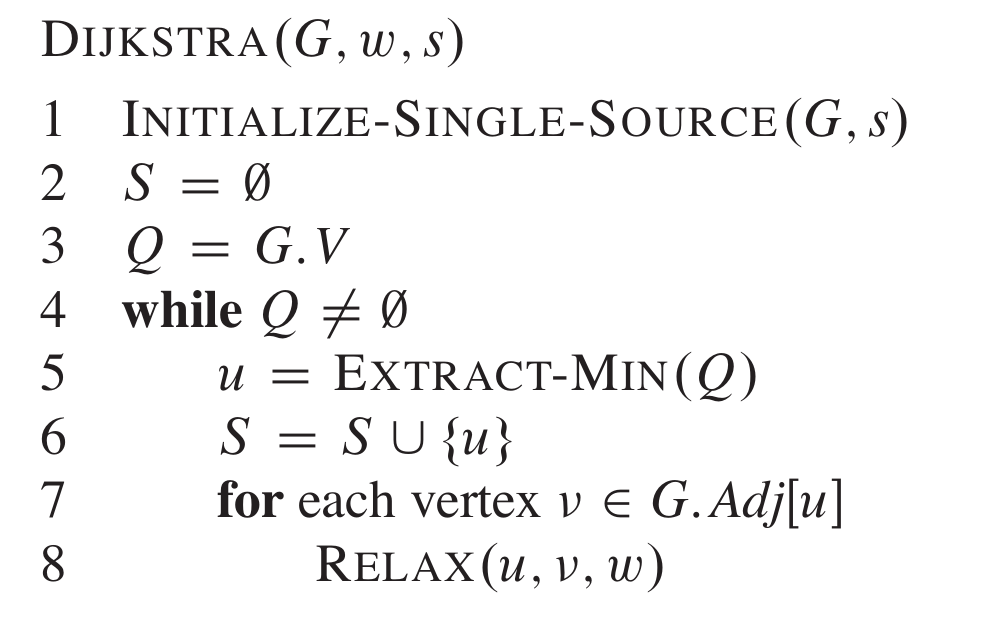
\includegraphics[width=0.5\textwidth]{dijkstra-code.png}
\end{figure}
In initialization, $d(s) = 0$ and the $d$ for the rest of nodes are $+\infty$. In relax function, if $d(v) > d(u) + w((u,v))$, set $d(v) = d(u) + w((u,v))$ and update the partent of $v$ if necessary.
\subsection{Time}
Line 5 will execute $|V|$ times and line 8 will execute $|E|$ times. Therefore
\[T = |V|T_{\text{extract-min}} + |E| T_{\text{decrease-key}}\]